\subsection{DQN with Cart Pole}
\textbf{Different network architectures} had clearly performance differences. The simplest network that contained one hidden layer and 24 neurons was not able to learn the task in 1000 episodes. From the figure \ref{fig:nn_24} we can see that it was close to reaching the average reward of 200 and it had strong upwards trend in the end. Learning only spiked upwards so the model avoided sudden drops in reward which happened more often with the other architectures.

\begin{figure}[H]
    \centering
    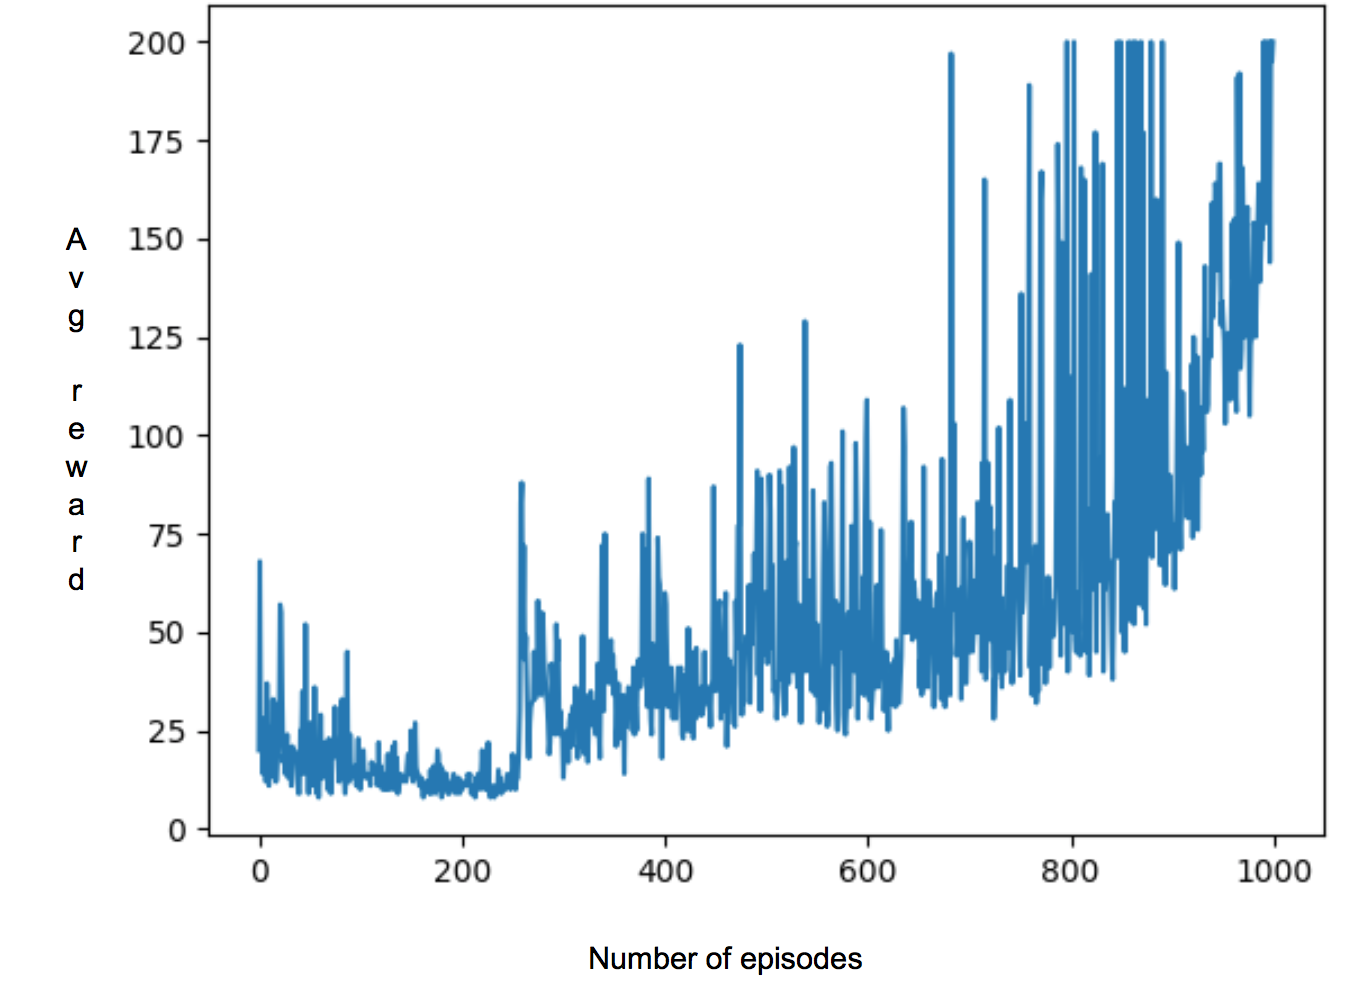
\includegraphics[width=0.4\textwidth]{images/nn_24.png}
    \caption{
    Episode rewards for architecture with one hidden layer with 24 neurons.
    }
    \label{fig:nn_24}
\end{figure}

The two more complex networks learned the task (the average reward was over 195) under 350 episodes. From figures \ref{fig:nn_24_24} and \ref{fig:nn_24_48} we can see that network with 24 neurons in both layers learned the task more generally. It didn't have huge drops in the reward that the more complex network had even after it had multiple successful episodes that achieved the maximum reward.

\begin{figure}[H]
    \centering
    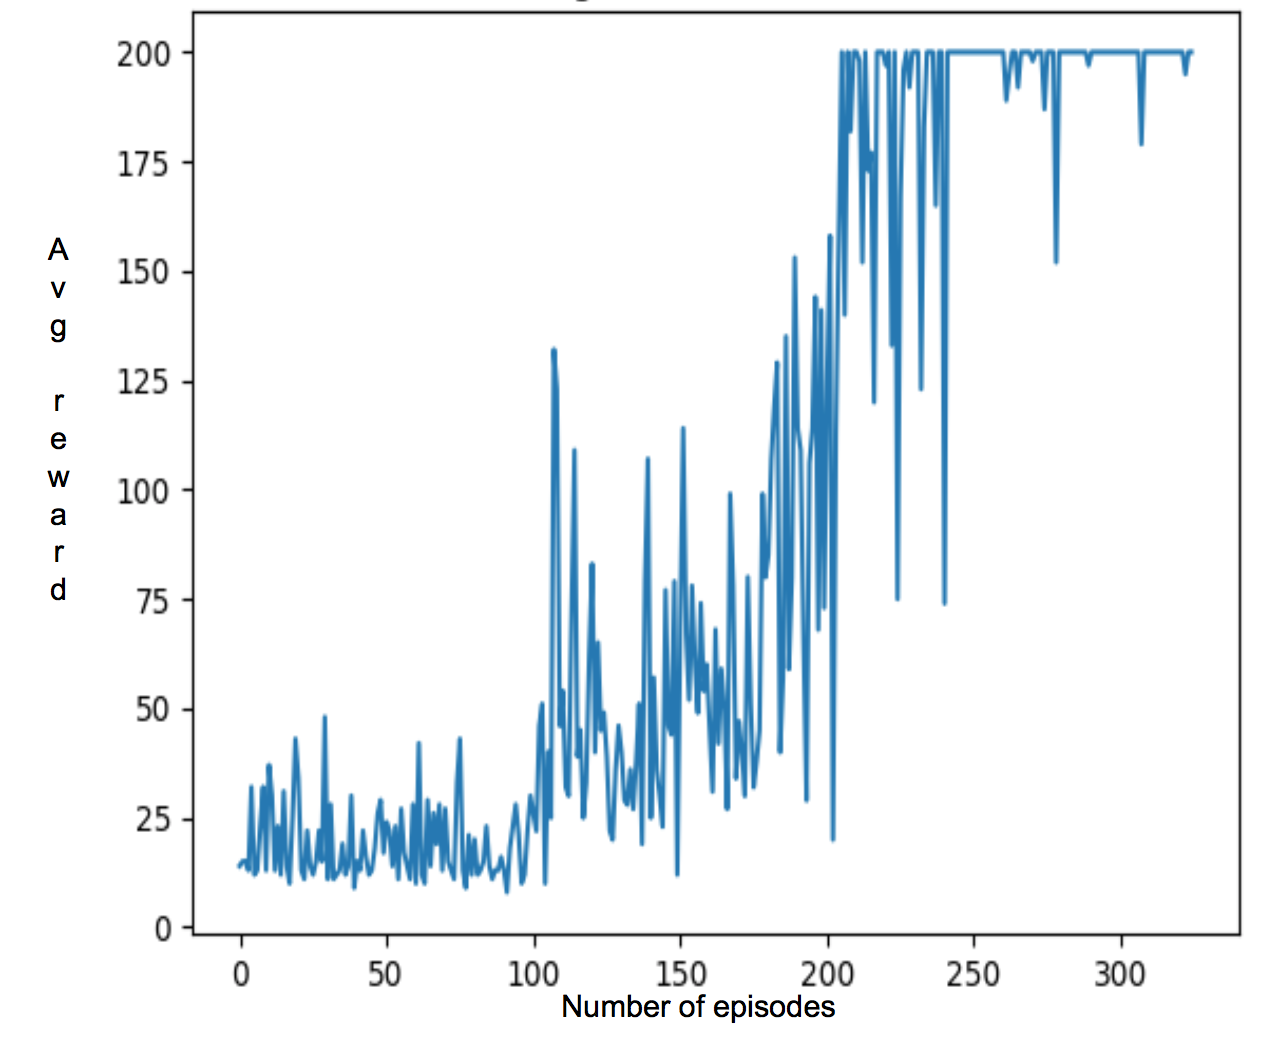
\includegraphics[width=0.4\textwidth]{images/nn_24_24.png}
    \caption{
    Episode rewards for architecture with two hidden layers with 24 neurons.
    }
    \label{fig:nn_24_24}
\end{figure}

\begin{figure}[H]
    \centering
    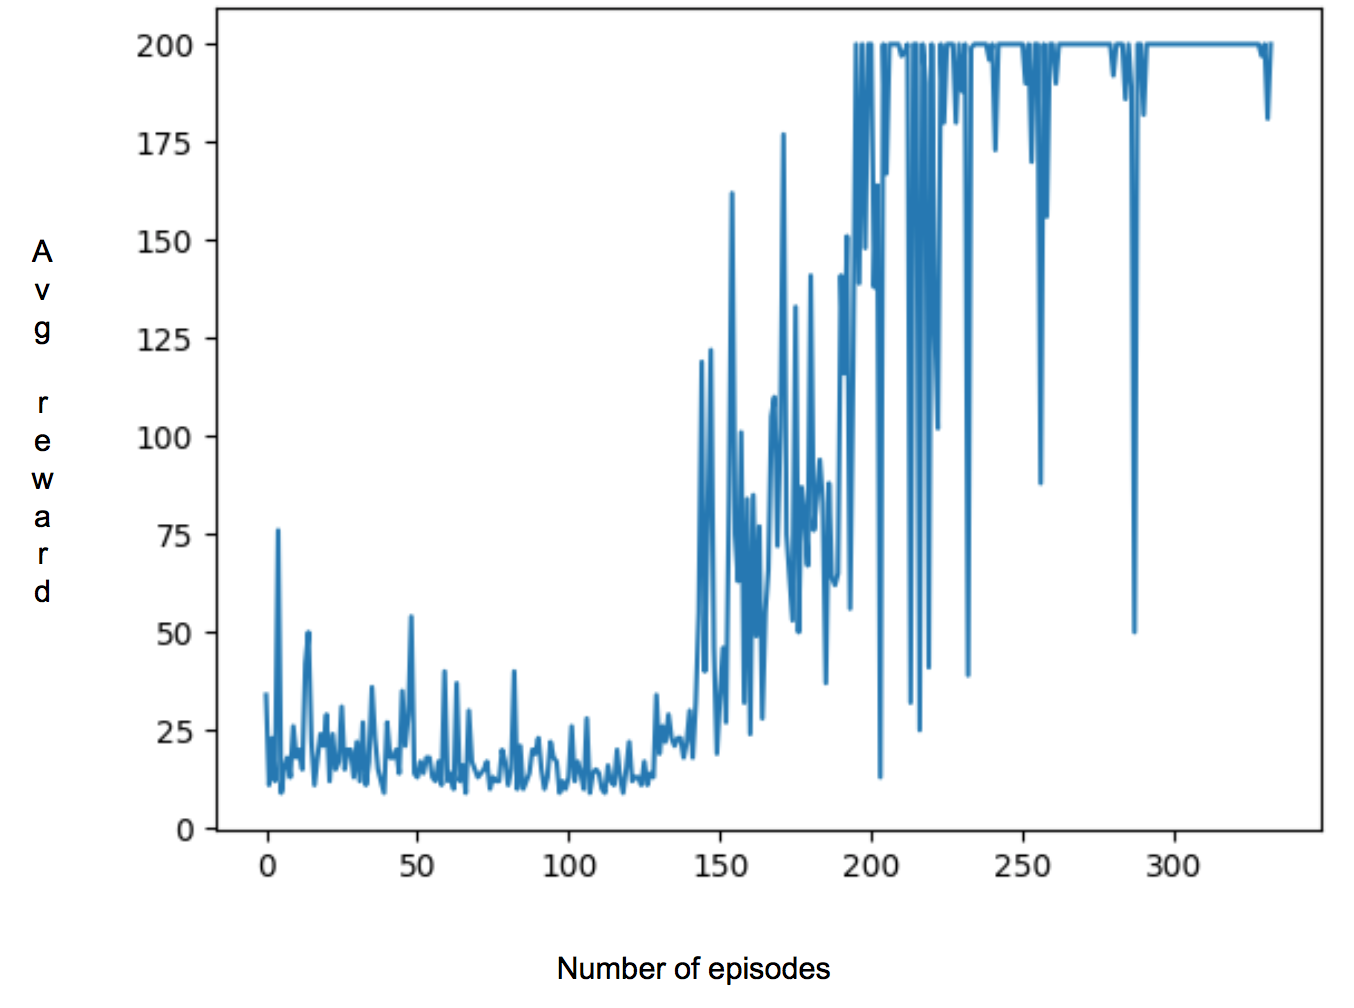
\includegraphics[width=0.4\textwidth]{images/nn_24_48.png}
    \caption{
    Episode rewards for architecture with two hidden layers from which the first had 24 neurons and the second 48.
    }
    \label{fig:nn_24_48}
\end{figure}

\textbf{Different $\epsilon$-greedy strategies} had the results we expected. When the algorithm was not able to explore enough it exploited a strategy that was a local minimum. As a result, the model was not able to reach maximum score.
With really eager $\epsilon$-greedy strategy, where $epsilon$ value was over 0.1 still after 1000 episodes, the model was not able to learn optimal strategy. Reasons is obvious - probability to take random action is very high (0.1). Results for this $epsilon$ value we can see from the figure \ref{fig:e-greedy}.
Best $\epsilon$-greedy strategy was achieved with the formula 5 that had the decay of 0.1.

\begin{figure}[H]
    \centering
    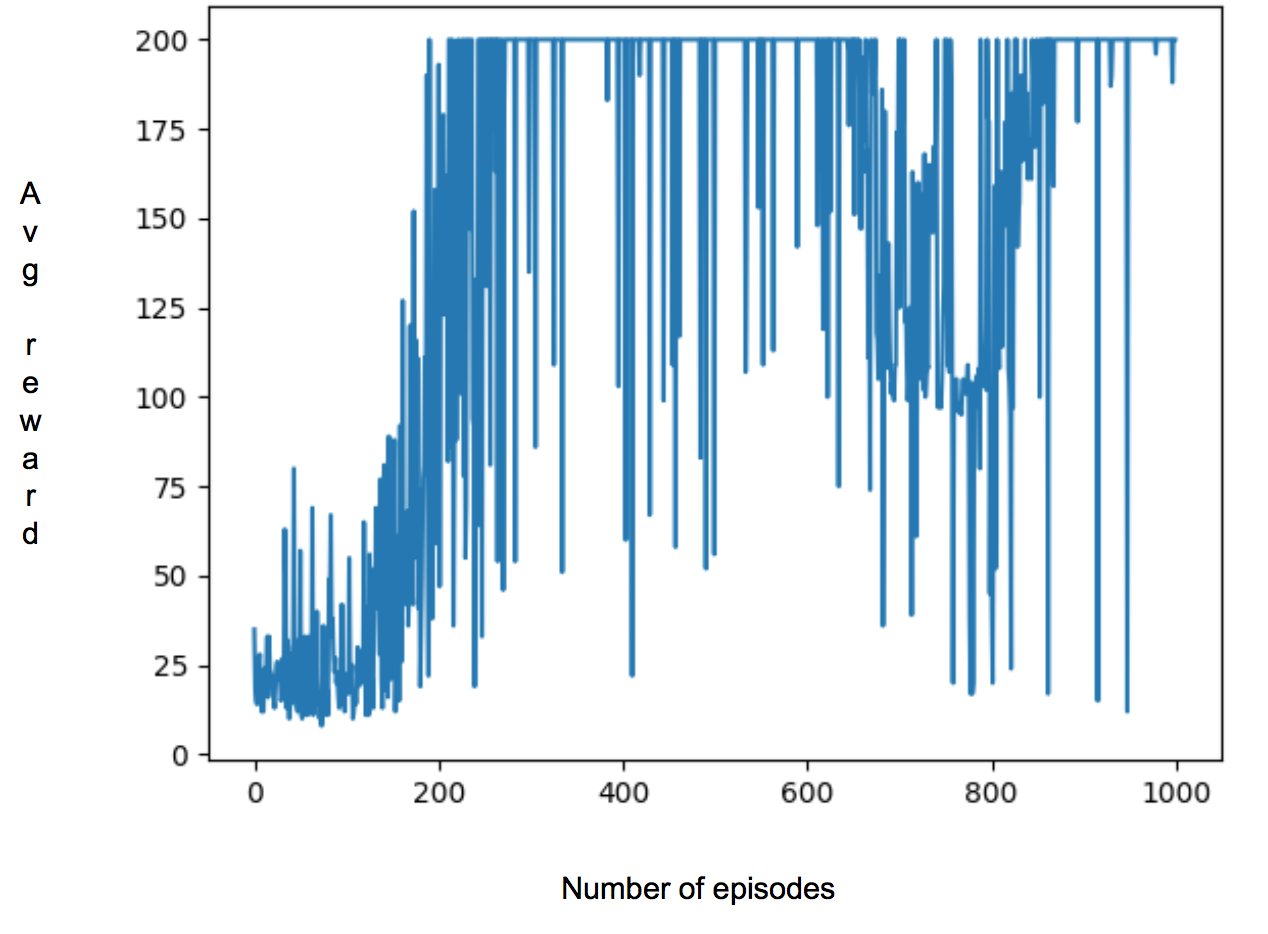
\includegraphics[width=0.4\textwidth]{images/e-greedy.png}
    \caption{
    Episode rewards for $\epsilon$-greedy strategy that had $\epsilon$ value over 0.1 for 1000 episodes. Decay value was 0.01 for the epsilon strategy in the formula 5.
    }
    \label{fig:e-greedy}
\end{figure}

\textbf{Different experience replay strategies} had also the results we expected. With a very small size of 2 model was not able to learn the task at all. With really high memory and batch size, it learned it really well. The only noticeable result was with the memory size of 1000. Intuitively we felt that 64 observations chosen randomly from 1000 would enough variation to break the strong correlation between close-by observations. This turned out to be not true like we can see from the figure \ref{fig:experience_replay}. Based on the figure model hasn't learned the task. It can achieve maximum score, but only for a short time. Then reward drops to almost zero. It seems that it learns a strategy, it utilizes it until it learns a completely new one. This cycle repeats and at least with 1000 episodes it hasn't learned any steady strategy.

\begin{figure}[H]
    \centering
    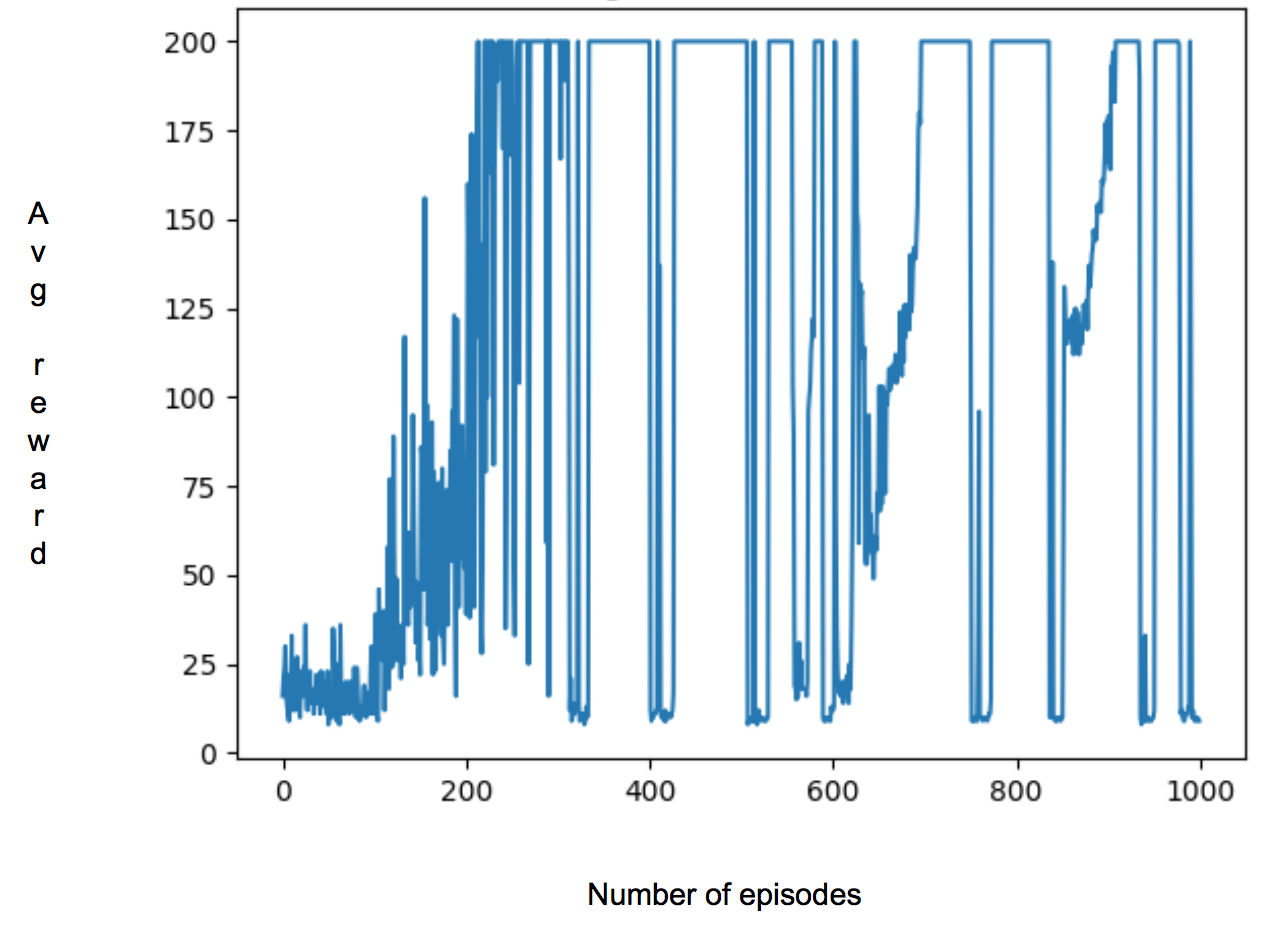
\includegraphics[width=0.4\textwidth]{images/experience_replay.png}
    \caption{
    Episode rewards when replay memory stored only the 1000 observations and had the batch size of 64.
    }
    \label{fig:experience_replay}
\end{figure}

Best results for Cart Pole where achieved with neural network that had two layers with 24 neurons. Formula 5 was used for $\epsilon$-greedy strategy with decay paramater of 0.1. Experience replay that helped the learning the most had memory size of 100000 and batch size of 64.
